
使用擦除函数(或erase-remove习惯用法)从vector中间删除项需要O(n)(线性)时间。因为元素必须从向量的末尾移动,以填补删除项之间的空白。若vector中项目的顺序不重要,就可以优化这个过程,使其花费O(1)(常数)时间。

\subsubsection{How to do it…}

这个方法利用了这样一个事实,即从vector的末尾删除一个元素是快速和简单的。

\begin{itemize}
\item 
让我们从定义一个函数来打印一个vector开始:

\begin{lstlisting}[style=styleCXX]
void printc(auto & r) {
	cout << format("size({}) ", r.size());
	for( auto & e : r ) cout << format("{} ", e);
	cout << '\n';
}
\end{lstlisting}

\item 
main()函数中,定义了一个int类型的vector,并使用printc()将其打印出来:

\begin{lstlisting}[style=styleCXX]
int main() {
	vector v{ 0, 1, 2, 3, 4, 5, 6, 7, 8, 9 };
	printc(v);
}
\end{lstlisting}

输出:

\begin{tcblisting}{commandshell={}}
size(10) 0 1 2 3 4 5 6 7 8 9
\end{tcblisting}

\item 
现在编写一个函数,从vector中删除一个元素:

\begin{lstlisting}[style=styleCXX]
template<typename T>
void quick_delete(T& v, size_t idx) {
	if (idx < v.size()) {
		v[idx] = move(v.back());
		v.pop_back();
	}
}
\end{lstlisting}

quick\_delete()函数有两个参数,一个vector v和一个索引idx。首先,检查索引是否在边界之内。然后,从<algorithms>头文件中调用move()函数将vector的最后一个元素移动到索引的位置。最后,调用v.pop\_back()函数从后面缩短vector。

\item 
还有一个版本的quick\_delete(),用于迭代器而非索引。

\begin{lstlisting}[style=styleCXX]
template<typename T>
void quick_delete(T& v, typename T::iterator it) {
	if (it < v.end()) {
		*it = move(v.back());
		v.pop_back();
	}
}
\end{lstlisting}

\item 
现在可以在main()函数中调用它:

\begin{lstlisting}[style=styleCXX]
int main() {
	vector v{ 12, 196, 47, 38, 19 };
	printc(v);
	auto it = std::ranges::find(v, 47);
	quick_delete(v, it);
	printc(v);
	quick_delete(v, 1);
	printc(v);
}
\end{lstlisting}

输出如下所示:

\begin{tcblisting}{commandshell={}}
size(5) 12 196 47 38 19
size(4) 12 196 19 38
size(3) 12 38 19
\end{tcblisting}

对quick\_delete()的第一次调用使用std::ranges::find()算法中的迭代器。这将从向量中删除值47。注意vector(19)后面的值取代了它的位置。第二次调用quick\_delete()使用索引(1)从vector(196)中删除第二个元素。同样,vector后面的值会取代其位置。
\end{itemize}

\subsubsection{How it works…}

quick\_delete()函数使用一个简单的技巧快速有效地从vector中删除元素。vector后面的元素会移动(而不是复制)到要删除的元素的位置。删除的元素在进程中丢弃。

然后,pop\_back()函数将vector从末尾开始缩短一个元素,即删除vector后面的元素开销很小。pop\_back()函数的操作复杂度不变,因为它只更改end()迭代器。

这个图显示了quick\_delete()操作前后vector的状态:

\hspace*{\fill} \\ %插入空行
\begin{center}
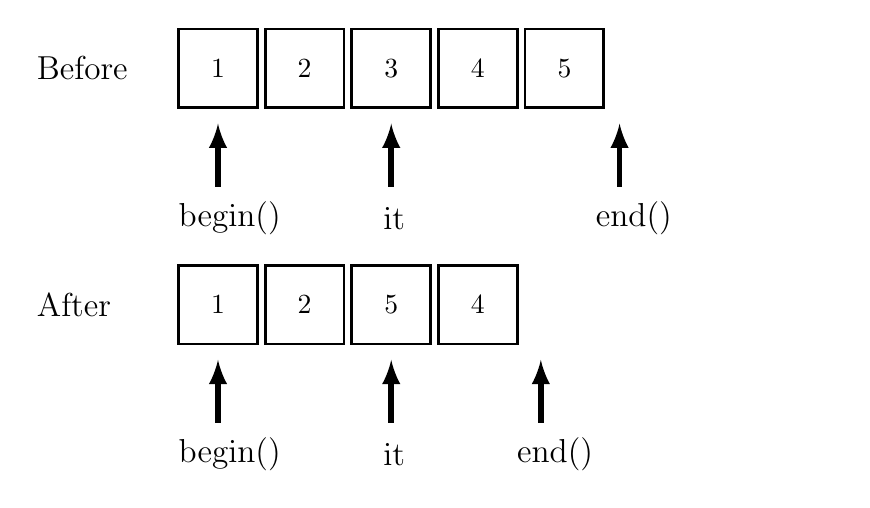
\begin{tikzpicture}
%before
\node[text width=3cm, font=\large] at (-0.3,0.5) {Before};

\foreach \x [evaluate=\x as \index using int(\x+1)] in {0,...,4} {
	\draw[line width=1pt] (1.1*\x,1) rectangle (1.1*\x+1,0) node[pos=.5] {\index};
}

\draw[line width=2pt][-latex] (0.5,-1.0) -- (0.5,-0.2);
\draw[line width=2pt][-latex] (2.7,-1.0) -- (2.7,-0.2);
\draw[line width=2pt][-latex] (5.6,-1.0) -- (5.6,-0.2);

\node[text width=3cm, font=\large] at (1.5,-1.4) {begin()};
\node[text width=3cm, font=\large] at (4.1,-1.4) {it};
\node[text width=3cm, font=\large] at (6.8,-1.4) {end()};

%after
\node[text width=3cm, font=\large] at (-0.3,-2.5) {After};
\draw[line width=1pt] (1.1*0,-3) rectangle (1.1*0+1,-2) node[pos=.5] {1};
\draw[line width=1pt] (1.1*1,-3) rectangle (1.1*1+1,-2) node[pos=.5] {2};
\draw[line width=1pt] (1.1*2,-3) rectangle (1.1*2+1,-2) node[pos=.5] {5};
\draw[line width=1pt] (1.1*3,-3) rectangle (1.1*3+1,-2) node[pos=.5] {4};

\draw[line width=2pt][-latex] (0.5,-4.0) -- (0.5,-3.2);
\draw[line width=2pt][-latex] (2.7,-4.0) -- (2.7,-3.2);
\draw[line width=2pt][-latex] (4.6,-4.0) -- (4.6,-3.2);

\node[text width=3cm, font=\large] at (1.5,-4.4) {begin()};
\node[text width=3cm, font=\large] at (4.1,-4.4) {it};
\node[text width=3cm, font=\large] at (5.8,-4.4) {end()};
\end{tikzpicture}

图3.4  quick\_delete()之前和之后
\end{center}

quick\_remove()操作只是将元素从vector的后面移动到迭代器(it)的位置,然后将vector缩短一个元素。使用std::move()而不是赋值来移动元素很重要,移动操作比复制赋值快得多,特别是对于大型对象。

若不需要有序元素,这是一种非常有效的技术。可以在常数(O(1))时间内完成,并不涉及到其他元素。









